% Author: Matt Toman

\chapter{History of Retinal Imaging}

\label{history_retinal_imaging}
\lhead{\emph{History of Retinal Imaging}}


\section{The History of Retinal Imaging}


Direct examination of the retina is prevented by the optical properties of the eye that enable image capture and formation.  That is to say, when trying to form a retinal image from outside via an inverse imaging transform, depiction of the retina is actually prevented by the nature of the original transform which results in a focused image on its surface.

If light is shined into the eye at a certain angle, a blurred reflection of the retina can make the pupil appear to be red in colour.  This is known as the red reflex, and has been understood for hundreds of years.  Obtaining a focused retinal image is much more difficult, however, and requires specialist techniques.  The first successful attempt to acquire a retinal image was performed by Jean Mery, a French physician, in 1704.  Mery  showed that if a live cat is submerged in water, the vessels of its retina can be seen from the outside.\cite{collegeoptometrists}

Czech scientist Jan Purkinje observed the fundus of a dog and later a human eye with the use of his myopic spectacles.  Acting as a concave mirror, they reflected light into the eye from a candle situated behind the subject.  His research resulted in the realisation of the first principles of the opthalmoscope in 1823.  This was later reinvented by Charles Babbage in 1845.\cite{flick1947centenary,keeler1997150}  Babbage was also responsible for the original concept of a programmable computer, solidifying the link between retinal imaging and computing at an early stage.\cite{halacy1970charles}

The opthalmoscope was reinvented again by von Helmholtz in 1851.  As with many other important inventions, it was not based on any radical new concepts, but was a combination of several known principles.  The fundamentals of opthalmoscopy are simple.  If the subject's eye is emmetropic, or sharp and well defined, light rays which emanate from a given point on the fundus will emerge as parallel beams.  When this beam enters the pupil of an emmetropic observer the individual rays are focused on to the observer's retina, as shown in \fref{fig:direct_opthal}.  The result is the formation of the image of the patient's retina on the observer's retina.  This is known as direct opthalmoscopy.

%\begin{figure}[htbp]
%\centering
%  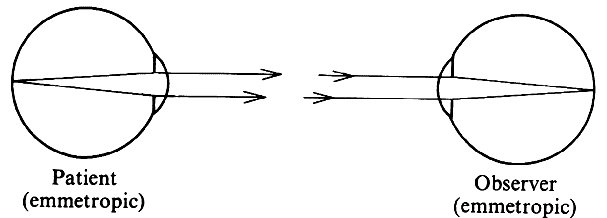
\includegraphics{figures/direct_opthalmoscopy}
%\caption{Imaging in direct ophthalmoscopy. Provided the subject and the observer are both emmetropic, rays emanating from a point in the subject's fundus will emerge as a parallel beam, focused on the observer's retina.\cite{colenbrander2013principles}}
%\label{fig:direct_opthal}
%\end{figure}


There is a significant problem with this method, however.  The patient's fundus has to be well illuminated for there to be sufficient light to visualise it.  Due to the optics of the eye, incident light can only reach the part of the fundus where the image of the light source falls.  Therefore the fundus can only be seen where the observed and illuminated areas overlap, and in the emmetropic eye this requires the light source and the observer's pupil to be optically aligned.

Fortunately there are several methods in which the illuminating and observing beams can be optically aligned, as shown in \fref{fig:illum_methods}.  The problem was solved by von Helmholtz with the use of a semireflecting mirror, made from thin pieces of glass in a parallel arrangement (A).  Epkens and Ruete used a perforated concave mirror (B), which places illuminating light rays around the observation beam.  Modern-day hand held instruments now use a small mirror or a prism, which utilises the bottom half of the subject's pupil for illumination and the top half for observation (C).


%\begin{figure}[htbp]
%\centering
%  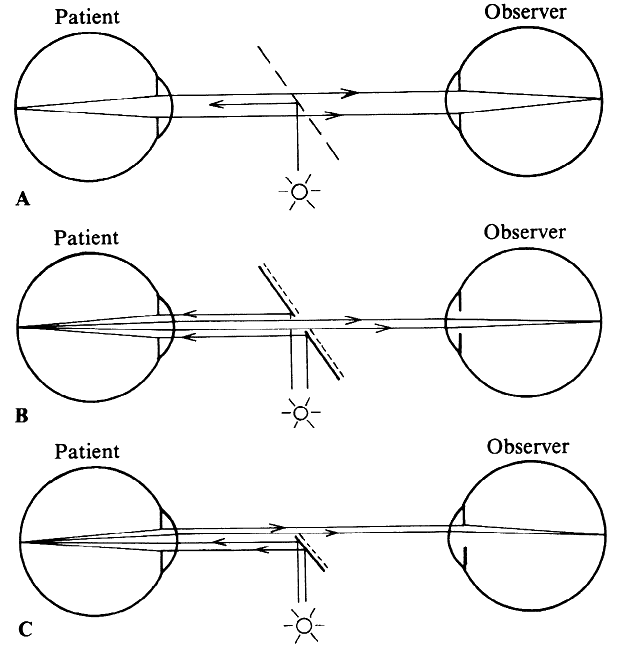
\includegraphics{figures/illumination_methods}
%\caption{Illumination methods in direct opthalmoscopy. A: Semireflecting mirror (Helmholtz). B: Perforated mirror (Epkens & Ruete). C: Prism (modern).\cite{colenbrander2013principles}}
%\label{fig:illum_methods}
%\end{figure}


The inspection and evaluation of the retina quickly became a routine excercise for ophthalmologists.  The first known image of the human retina, shown below in \fref{fig:human_retina} was published by the Dutch ophthalmologist van Trigt in 1853.  Previously, Purkinje had provided sketches of his own retinal vascalature, shown in \fref{fig:retinal_drawings}.

%\begin{figure}[htbp]
%\centering
%  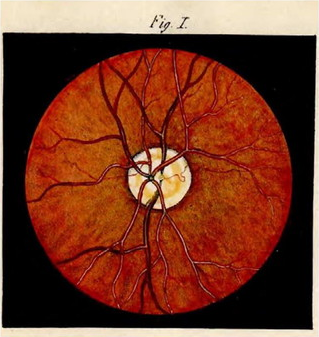
\includegraphics{figures/first_human_retina}
%\caption{First known image of the human retina, drawn by Van Trigt in 1853.\cite{van1853dissertatio}}
%\label{fig:human_retina}
%\end{figure}
%
%\begin{figure}[htbp]
%\centering
%  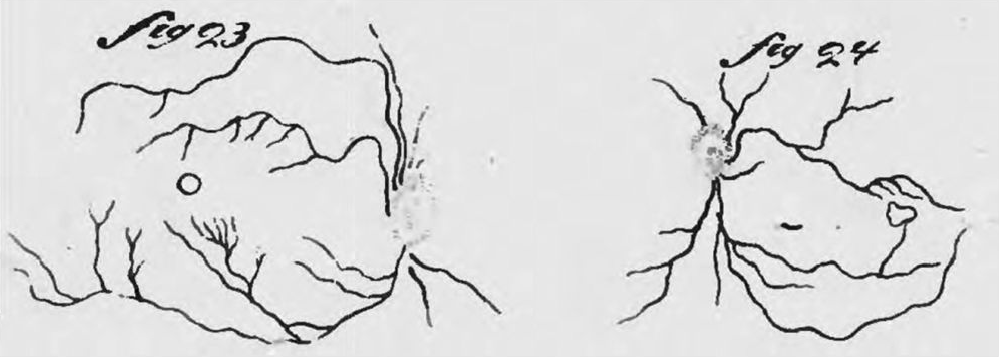
\includegraphics{figures/retinal_vasc_drawings}
%\caption{Early drawings of retinal vasculature, published by Purkinje in 1823.}
%\label{fig:retinal_drawings}
%\end{figure}

Due to the high prevalence of infectious diseases at the time, and because the ophthalmoscope necessitated the physician to be in close contact with the face of the patient, it became popular to image the eye photographically.  The first clear photographic images of the retina were obtained by German opthalmologist Gerloff in 1891.\cite{gerloffphoto}  In 1910, a Swede named Gullstrand developed the fundus camera.  He went on to receive the Nobel prize for his invention, and the concept is still utlised to image the retina in the present day.\cite{gullstrandcamera}  It has remained the primary method of retinal imaging because of how cost effective and safe it is to use.  

The next crucial development was the invention of fluorescein angiographic imaging.  A flueroescent dye is injected into the bloodstream and binds to the patient's leukocytes.\cite{novotny1961method}  A fundus camera with additional narrow band filters can then be used to capture the image.  This method has led to a better understanding of the function of retinal circulation.  However, concerns over safety have resulted in this method being slowly replaced by tomographic imaging for its primary uses, namely treatment of macular edema and macular degeneration. .

A serious limitation of fundus photography is that it only obtains a 2D representation of 3D retinal tissues, projected onto the imaging plane.  Stereo fundus photography was first described in 1964 by Allen.\cite{allen1964ocular}  This new approach relied on multi-angle retinal images combined by the human observer to derive a 3D shape.  Confocual scanning laser opthalmoscopy was later developed.  This innovation utilised a confocal aperture to obtain multiple images of the retina at different depths, yielding an estimate of its 3D shape.  Unfortunately the optics of the eye limit the depth of resolution of confocal imaging to only 100 μm, which is inadequate when compared with the typical thickness of the whole retina (300-500$\mu m$).\cite{webb1987confocal}

Tomographic imaging of the retina has become common practice following the development of femtosecond lasers, super-luminescent diodes, and, most significantly, the application of optical coherence tomography (OCT) to retinal imaging.\cite{huang1991optical}  This technique uses light to capture 3D images from within optical scattering media at micrometer-resolution, allowing for true 3D optical sectioning of the retina.\cite{van2007recent}
\section{The History of Retinal Image Processing}


Retinal image analysis methods were first examined by Matsui et al.  Their approach was grounded in mathematical morphology, utilising digitized slides of fluorescein angiograms of the retina, with a primary focus on vessel segmentation.\cite{matsui1973study}  

Many attempts to segment other anatomical structures in the eye were made in the subsequent years, all based on the use of digitized slides.  Badouin et al were the first to provide a method to detect and segment abnormal ocular structures.  In 1984 they described an image analysis method for the detection of microaneurysms, which is a characteristic symptom of diabetic retinopathy.\cite{baudoin1983automatic}  Their approach also utilised digitized angiographic images.  Microaneurysms were detected via the use of a "top-hat" transform, a step-type varient of a digital image filter.\cite{sonka1998image}  

The field of retinal image analysis changed drastically in the 1990s with the development of digital retinal imaging and filter-based image analysis techniques.  These advances in digital-based technology resulted in rapidly increasing numbers of publications.